% bei Standalone in documentclass noch:
% \RequirePackage{luatex85}

\documentclass[captions=tableheading, titlepage= firstiscover, parskip = half , bibliography=totoc]{scrartcl}
%paper = a5 für andere optinen
% titlepage= firstiscover
% bibliography=totoc für bibdateien
% parskip=half  Veränderung um Absätze zu verbessern

\usepackage{scrhack} % nach \documentclass
\usepackage[aux]{rerunfilecheck}
\usepackage{polyglossia}
\usepackage[style=numeric, backend=biber]{biblatex} % mit [style = alphabetic oder numeric] nach polyglossia
\addbibresource{lit.bib}
\setmainlanguage{german}

\usepackage[autostyle]{csquotes}
\usepackage{amsmath} % unverzichtbare Mathe-Befehle
\usepackage{amssymb} % viele Mathe-Symbole
\usepackage{mathtools} % Erweiterungen für amsmath
\usepackage{fontspec} % nach amssymb
% muss ins document: \usefonttheme{professionalfonts} % für Beamer Präsentationen
\usepackage{longtable}

\usepackage[
math-style=ISO,    % \
bold-style=ISO,    % |
sans-style=italic, % | ISO-Standard folgen
nabla=upright,     % |
partial=upright,   % /
]{unicode-math} % "Does exactly what it says on the tin."
\setmathfont{Latin Modern Math}
% \setmathfont{Tex Gyre Pagella Math} % alternativ

\usepackage[
% die folgenden 3 nur einschalten bei documenten
locale=DE,
separate-uncertainty=true, % Immer Fehler mit ±
per-mode=symbol-or-fraction, % m/s im Text, sonst \frac
]{siunitx}

% alternativ:
% per-mode=reciprocal, % m s^{-1}
% output-decimal-marker=., % . statt , für Dezimalzahlen

\usepackage[
version=4,
math-greek=default,
text-greek=default,
]{mhchem}

\usepackage[section, below]{placeins}
\usepackage{caption} % Captions schöner machen
\usepackage{graphicx}
\usepackage{grffile}
\usepackage{subcaption}

% \usepackage{showframe} Wenn man die Ramen sehen will

\usepackage{float}
\floatplacement{figure}{htbp}
\floatplacement{table}{htbp}

\usepackage{mhchem} %chemische Symbole Beispiel: \ce{^{227}_{90}Th+}


\usepackage{booktabs}

 \usepackage{microtype}
 \usepackage{xfrac}

 \usepackage{expl3}
 \usepackage{xparse}

 % \ExplSyntaxOn
 % \NewDocumentComman \I {}  %Befehl\I definieren, keine Argumente
 % {
 %    \symup{i}              %Ergebnis von \I
 % }
 % \ExplSyntaxOff

 \usepackage{pdflscape}
 \usepackage{mleftright}

 % Mit dem mathtools-Befehl \DeclarePairedDelimiter können Befehle erzeugen werden,
 % die Symbole um Ausdrücke setzen.
 % \DeclarePairedDelimiter{\abs}{\lvert}{\rvert}
 % \DeclarePairedDelimiter{\norm}{\lVert}{\rVert}
 % in Mathe:
 %\abs{x} \abs*{\frac{1}{x}}
 %\norm{\symbf{y}}

 % Für Physik IV und Quantenmechanik
 \DeclarePairedDelimiter{\bra}{\langle}{\rvert}
 \DeclarePairedDelimiter{\ket}{\lvert}{\rangle}
 % <name> <#arguments> <left> <right> <body>
 \DeclarePairedDelimiterX{\braket}[2]{\langle}{\rangle}{
 #1 \delimsize| #2
 }

\setlength{\delimitershortfall}{-1sp}

 \usepackage{tikz}
 \usepackage{tikz-feynman}

 \usepackage{csvsimple}
 % Tabellen mit \csvautobooktabular{"file"}
 % muss in table umgebung gesetzt werden


% \multicolumn{#Spalten}{Ausrichtung}{Inhalt}

\usepackage{hyperref}
\usepackage{bookmark}
\usepackage[shortcuts]{extdash} %nach hyperref, bookmark

\newcommand{\ua}[1]{_\symup{#1}}
\newcommand{\su}[1]{\symup{#1}}


\title{Versuch 353}
\subtitle{Das Relaxationsverhalten eines LC-Kreises}
\author{Sebastian Pape\\
        sepa@gmx.de \and
        Jonah Nitschke\\
        lejonah@web.de}
\date{Durchführung: 24.01.2017\\
      Abgabe: 31.01.2017}

\begin{document}
\maketitle
\setcounter{page}{1}

\section{Theorie}

In dem Versuch V353 wurde das Relaxationsverhalten eines $RC$-Kreises untersucht.
Relaxation bedeutet, dass ein System aus seinen Ruhezustand gebracht wird
und nicht-oszillatiorisch in diesen zurückkehrt.
Mit einem $RC$-Kreis ist solch ein Relaxationsverhalten zu erreichen.

\subsection{Ent- und Aufladevorgang}

Bei dem Ladevorgang eines Kondensators mit der Kapazität $C$ über einen Widerstand
$R$ lässt sich die Ladung auf dem Kondensator als Funktion der Zeit darstellen.
Es ergibt sich unter der Randbedingung $Q(\infty) = 0$ die folgende Formel.

\begin{equation}
  \label{eqn:Entladen}
  Q(t) = Q(0)\cdot \exp{(-\frac{t}{RC})}
\end{equation}

Für den Aufladevorgang gelten die Randbedingungen $Q(0) = 0$ und $Q(\infty) = CU_0$. Dabei ist $U_0$ die Spannung der Spannungsquelle. Damit ergibt sich
die folgende Formel des Aufladevorgangs eines Kondensators über einen Widerstand.

\begin{equation}
  \label{eqn:aufladen}
  Q(t) = CU_0(1 - \exp{(-\frac{t}{RC})})
\end{equation}

$RC$ wird auch \emph{spezifische Zeitkonstante} genannt, da dieser Ausdruck ein Maß
der Geschwindigkeit des Entladevorgangs darstellt.
Nach $\tau = RC$ ändert sich die Ladung des Kondensators um den Faktor $0,368$. Nach $2,3\tau$ sind nur noch 10\% des Ausgangswertes der Ladung auf dem
Kondensator vorhanden.

\subsection{Relaxationsverhalten bei periodischer Anregung}

Wird nun an den $RC$-Kreis eine periodische Spannung $U(t) = U_0\cos{\omega t}$
anstelle einer einzelnen Erregung angelegt ändert sich das Relaxationsverhalten
mit der Frequenz $\omega$. Ist $\omega \ll \frac{1}{RC}$ sind die
Spannungen des Generators und des Kondensators näherungsweise in Phase.
Je hochfrequenter die Spannung wird, desto deutlicher wird die Phase
zwischen den beiden Spannungen.
Für $\omega\rightarrow\infty$ nähert sich die Phasenverschiebung asymptotisch
den Wert $\frac{\pi}{2}$.

\subsection{Der RC-Kreis als Integrator}

Mit Hilfe eines $RC$-Kreises lässt sich die angeschlossene Spannung $U(t)$
unter der Voraussetzun $\omega\ll\frac{1}{RC}$ integireren. Dies hängt damit zusammen, dass die Kondensatorspannung $U_C(t)$
proportional mit dem Integral von $U(t)$ zusammenhängt.
Unter der gestellten Bedingung gilt näherungsweise der Zusammenhang

\begin{equation}
  \label{eqn:Integrator}
  U_C(t) = \frac{1}{RC}\int_0^tU(t')\symup{d}t'.
\end{equation}

Daran ist erkenntlich, dass sich die Kondensatorspannung $U_C(t)$ als Integrator
der Generatorspannung $U(t)$ eignet.

\section{Durchführung}

Zu Beginn des Versuches wurde der $RC$-Kreis aufgebaut. Eine Schaltplanskizze
ist in Abb. \ref{fig:Aufbau} zu sehen.
Mit dieser Schaltung konnte der Auf- und Entladevorgangs des Kondensators
über das Oszilloskop beobachtet werden. Dazu wurde der Generator auf den
Rechteckspannungsbetrieb eingestellt und das Oszilloskop so geregelt, dass
die Lage des Spannungsnullpunktes zu sehen ist. Während des Suchvorganges des
Spannungsnullpunktes wurde die Periodendauer der Rechteckspannung möglichst groß gewählt. Sobald eine geeignete Kurve gefunden wurde, konnte diese
als Bild gespeichert werden.

Danach wurde der Generator auf den Sinusspannunsbetrieb umgestellt, sodass
der $RC$-Kreis bei variirender Frequenz untersucht werden konnte.
Die Amplitude der Kondensatorspannung wurde bei insgesamt 15 verschiedenen
Frequenzen beobachtet. Dabei wurden fünf Frequenzen aus dem nieder
frequenten Bereich zwischen $10$ bis $\SI{100}{\hertz}$ betrachtet. Die
anderen zehn Frequenzen wurden aus dem Frequenzbereich zwischen $200$ bis
$\SI{1100}{\hertz}$ in hunderter Schritten gewählt. Bei der Messung wurden
neben der Frequenz und Kondensatorspannung auch die Generatorspannungen betrachtet.

Desweiteren wurde der Phasenunterschied zwischen Generator- und Kondensatorspannung
in Abhängigkeit von der Frequenz gemessen. Dafür wurden die beiden Spannungen
auf die Eingänge des Oszilloskops gelegt. Es wurde der Abstand der beiden
Nulldurchgänge, sowie die Periodendauer der Generatorspannung mit Hilfe
des digitlen Periodendauermessgerät, welches in dem Oszilloskop integriert ist
gemessen.

Abschließend wurde die Eigenschaft der Kondensatorspannung als Integrator
der Generatorspannung untersucht. Dafür wurde die Frequenz minimal gereglt,
sodass sie der Bedingung $\omega\ll \frac{1}{RC}$ genügt. Bei dem verwendeten
Generator war die Minimalfrequenz bei ca. $\SI{4}{\hertz}$ erreicht.
Nun wurde die Generatorspannung parallel zu der Kondensatorspannung auf dem
Oszilloskop ausgegeben und bei geeigneten Einstellungen als Bild gespeichert.
Die Messung wurde mit eines Sinusspannung, einer Rechteckspannung und einer
Dreieckspannung durchgeführt.\\

\FloatBarrier
\begin{figure}
  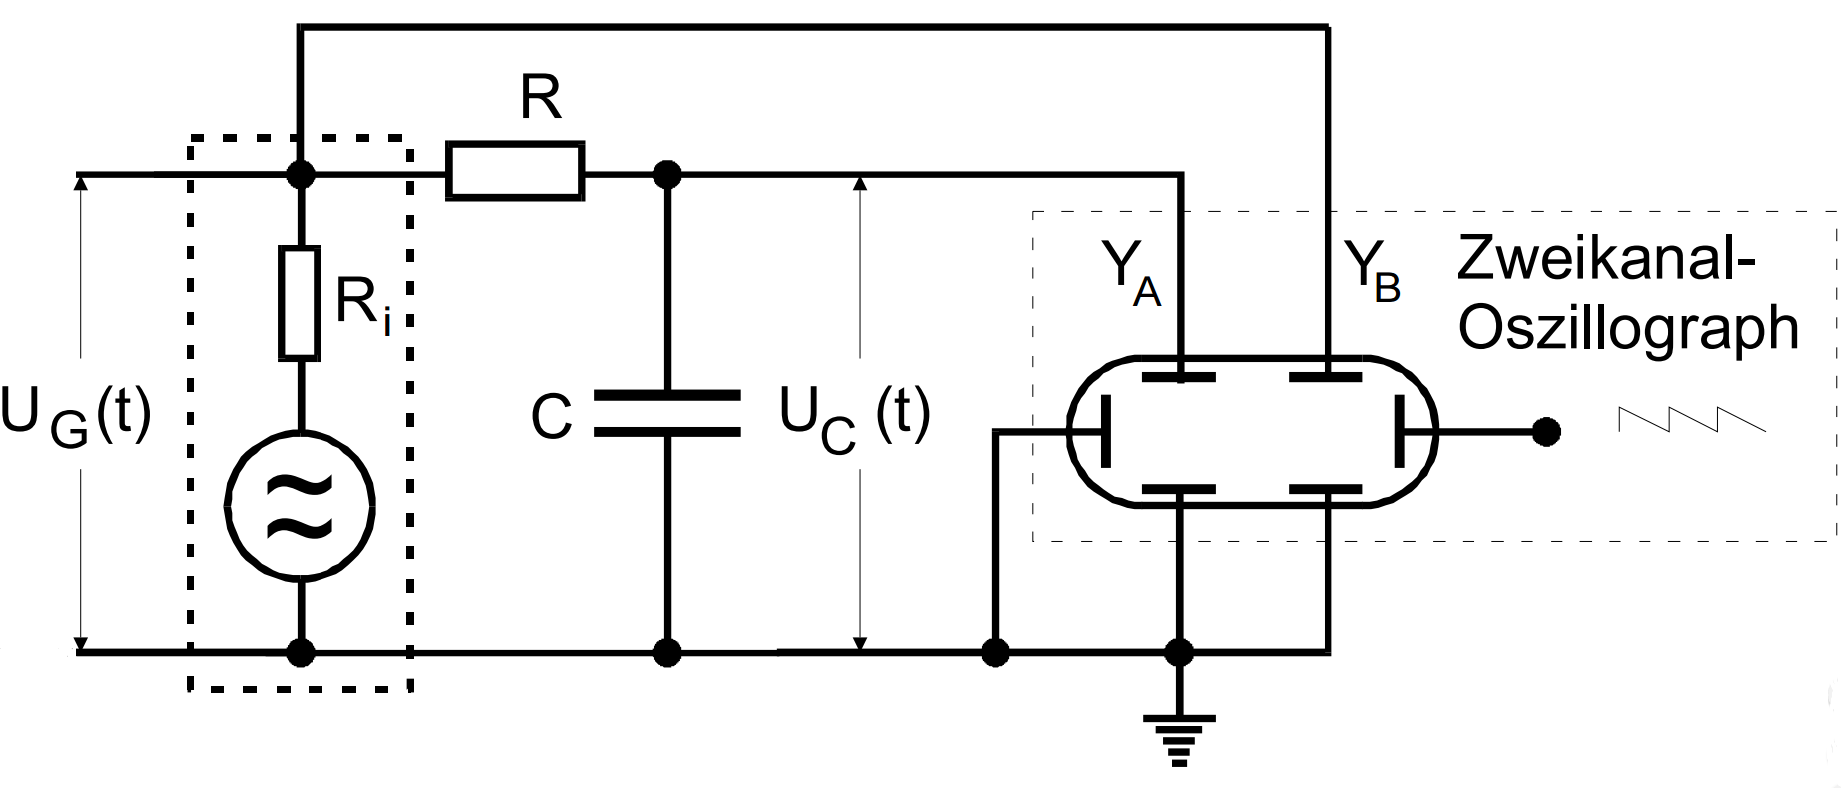
\includegraphics[width=\textwidth]{Aufbau_V353.PNG}
  \caption{Schaltplanskizze des verwendeten RC-Kreises}
  \label{fig:Aufbau}
\end{figure}

\end{document}
